\documentclass[11pt, a4paper]{article} 
\usepackage[polish]{babel}
\usepackage{longtable}
\usepackage{booktabs}
\usepackage{dcolumn}
\usepackage{geometry} % to change the page dimensions
\usepackage{graphicx} % support the \includegraphics command and options
\usepackage{float}
\usepackage{array} % for better arrays (eg matrices) in maths
\usepackage{verbatim} % adds environment for commenting out blocks of text & for better verbatim
\usepackage{lscape}
\usepackage{latexsym}
\usepackage{multirow}
\usepackage{amsmath}
\usepackage{makecell}
\let\lll=\amslll
%\savesymbol{lll}
\usepackage{amssymb}

%\usepackage{fontspec}
%\usepackage[utf8]{fontenc}
\usepackage[OT4]{fontenc}
\usepackage[utf8]{inputenc}

\usepackage{pdflscape} 
\usepackage{epstopdf}
\usepackage{pdfpages}

\setlength\parindent{0pt}

\newcommand{\HRule}{\rule{\linewidth}{0.5mm}}
\newcommand{\linia}{\rule{\linewidth}{0.1mm}}
\usepackage[  
  bookmarks=true,  
  bookmarksnumbered=false,  
  unicode=true,  
  pdftitle={Projekt zespołowy},
  pdfauthor={Paweł Bogner, Krzysztof Nomejko, Grzegorz Maj,
  Bartosz Folta, Marcin Dmochowski},
  pdfnewwindow=true,
  colorlinks=false
]{hyperref} 

\begin{document}
	%%%%%%%%%%%%%%%%%%%%%%%%%%%%%%%%%%%
% Strona tytułowa
%\newcommand{\HRule}{\rule{\linewidth}{0.5mm}}
\begin{titlepage}
  \begin{center}
    
    % Upper part of the page
    %\centering{\includegraphics[width=0.2\textwidth]{logo.png}\\[1cm]}

    \textsc{\Large Systemy zdarzeniowe}\\[3cm]
    
    % Title
    \centering{\HRule \\[0.5cm]}
	      {\LARGE  \textsc{Raport}\\[0.4cm]}
	      {\Large Opracowanie rozproszonego systemu koordnacji
                agentów mobilnych}
	      \centering{\HRule \\[1.5cm]}
	      
	      % Autor i prowadzący
	      \begin{minipage}{0.4\textwidth}
	        \begin{flushleft} \large
	          \emph{Skład grupy:}\\
	          Paweł \textsc{Bogner} \\
	          Marcin \textsc{Dmochowski} \\
	          Bartosz \textsc{Folta} \\	
	          Grzegorz \textsc{Maj} \\
	          Krzysztof \textsc{Nomejko} \\
		  
		  
	        \end{flushleft}
	      \end{minipage}
	      \begin{minipage}[b]{0.4\textwidth}
	        \begin{flushright} \large
		  \emph{Prowadzący:} \\
		  dr~inż. E.~\textsc{Roszkowska}
	        \end{flushright}

	      \end{minipage}
	      \vfill
	      % Bottom of the page
	          {\large \today}

  \end{center}
\end{titlepage}
%%%%%%%%%%%%%%%%%%%%%%%%%%%%%%%%%%%

	
	\section{Zarządzanie projektem}
\noindent Podczas realizacji projektu wykorzystano tradycyjną, płaską strukturę
zarządzania z jednym liderem (koordynatorem). Do zadań lidera należało
podejmowanie krytycznych decyzji projektowych, rozstrzyganie sporów
oraz kontrolowanie postępu prac nad przydzielonymi zadaniami.
\\\\
\noindent W kwestii rozstrzygania sporów, strona konfliktu ma prawo do
przedstawienia problemu na forum grupy, w celu jego wspólnego
przedyskutowania. W świetle przedstawionych argumentów i poglądów
lider ma obowiązek podjąć decyzję rozstrzygającą.
\\\\
\noindent Do przewidzianych środków komunikacji zdalnej należą \textit{Google
groups} oraz rozmowy telefoniczne. W celu składowania i
wymiany dokumentów zostanie wykorzystane oprogramowanie \textit{git}.
Każdy z członków grupy ma obowiązek korzystać z tego programu.
\\\\
\noindent Uznano, że każdy członek grupy zostanie obdarzony prawami własności
intelektualnej do części projektu, za której zrealizowanie był odpowiedzialny.


%\includepdf[landscape]{img/gantt.pdf}

	\section{Opis logiki}

kilka zdań

\begin{enumerate}
  \item pobranie informacji początkowych od serwera: współrzędne
    sektora początkowego,

  \item wysłanie zapytania o pozwolenie wjazdu do kolejnego
    sektora, \label{zapytanie}

  \item oczekiwanie na pozwolenie, przy jednoczesnym poruszaniu się
    zgodnie z wektorem wyznaczonym przez pola potencjałów,
    
  \item otrzymanie pozwolenia na wjazd do kolejnego sektora,
    ustawienie przeciwnego potencjału na ścianie sąsiadującej z
    kolejnym sektorem, otrzymanie współrzędnych następnego sektora
    docelowego,

  \item przejazd do kolejnego sektora,

  \item zwolnienie poprzedniego sektora, przejście do punktu \ref{zapytanie} 

\end{enumerate}





	\section{Zachowanie robotów wewnątrz pola}
	Zachowanie robotów wewnątrz pola zamodelowane jest za pomocą metody sztucznych pól potencjałów. Potencjały ustalane są w następujący sposób:
	\begin{itemize}
		\item robot oczekujący na zezwolenie wyjazdu z pola widzi wszystkie ściany jako spolaryzowane ładunkiem o znaku zgodnym ze znakiem jego ładunku (rys. \ref{pic:waiting}), a jego wektor sił ma składowe opisane następującymi równaniami:
                  $$F_x= A*((X-x)^2 - x^2)$$
		  $$F_y= A*((Y-y)^2 - y^2),$$
		\item robot wykonujący manewr przejazdu do innego pola widzi dodatkowy ładunek na ścianie, w kierunku której ma zmierzać (umieszczony z jej prawej strony, aby zapobiegać kolizjom) (rys. \ref{pic:moving}), a do składowych jego wektora sił dodaje się człon odpowiedzialny za modelowanie dodatkowego potencjału:
                  $$F_{xM}= +\frac{B}{(X_p-x)^2}$$
                  $$F_{yM}= +\frac{B}{(Y_p-y)^2},$$
		\item dwa roboty znajdujące się w tym samym polu zawsze są spolaryzowane ładunkami punktowymi o jednakowych znakach (rys. \ref{pic:tworobots}), a do wektora sił dodawany jest w tym wypadku następujący człon modelujący siłę wzajemnie je odpychającą:
                  $$F_{xD}= +\frac{C}{\mathrm{sgn}(x-x_D)(x-x_D)^2}$$
                  $$F_{yD}= +\frac{C}{\mathrm{sgn}(y-y_D)(y-y_D)^2},$$ 
		\item w wypadku, jeśli w polu znajdują się dwa roboty, każdy widzi inną polaryzację ścian -- taką, aby zgadzała się ona z jego stanem ruchu (oczekiwanie, zezwolenie na przejazd),
                \item przykład --- kiedy w polu znajdują się dwa roboty i robot, dla którego obliczamy wypadkowy wektor sił, wyjeżdża z pola, składowe jego sił opisane są nastepującymi równaniami:
                  $$F_x= A((X-x)^2 - x^2)+B(X_p-x)^2+C(x-x_D)^2$$
                  $$F_y= A((Y-y)^2 - y^2)+B(Y_p-y)^2+C(y-y_D)^2.$$ 
	\end{itemize}
	
	\begin{figure}[H]
		\centering
		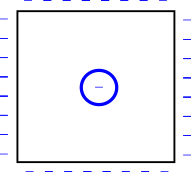
\includegraphics[scale=0.9]{img/waiting.png}
		\caption{Robot oczekujący na pozwolenie na wyjazd z komórki}
		\label{pic:waiting}
	\end{figure}
	\begin{figure}[H]
		\centering
		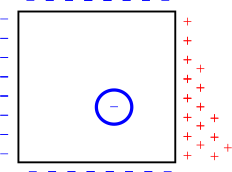
\includegraphics[scale=0.9]{img/moving.png}
		\caption{Robot wyjeżdżający z komórki}
		\label{pic:moving}
	\end{figure}
	\begin{figure}[H]
		\centering
		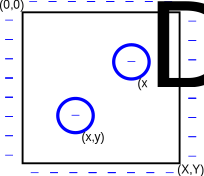
\includegraphics[scale=0.9]{img/tworobots.png}
		\caption{Dwa roboty oczekujące na pozwolenie na wyjazd z pola}
		\label{pic:tworobots}
	\end{figure}

	
\section{Zarys struktur danych}

\subsection{Scena}

W zrealizowanym modelu scena (plansza) jest strukturą, zawierającą tablicę komórek. Składa się ona na wszystkie 
niezbędne dane do sterowania robotami.\\

Pojedyncza komórka zawiera informacje o swoich wymiarach oraz listę wskaźników na roboty, które aktualnie się w niej znajdują, a także interfejs do dodawania i usuwania robotów w zależności od pojawiających się zdarzeń (roboty wjeżdżają i wyjeżdżają z komórki).\\

Klasa opisująca pojedynczego robota zawiera informacje o położeniu robota, jego prędkościach, a także niezbędne metody do wyliczania sił sterujących robotem (zależnych od położenia robota względem środka sektora i położenia ewentualnego drugiego robota w sektorze).

\subsection{Dane wymieniane z serwerem}

Serwer ma zadanie planowania tras dla robotów, wobec czego pożądana informacja dla każdego z robotów to następna komórka, do której ten ma się kierować oraz zezwolenie bądź brak zezwolenia na wjazd do niej. W przypadku braku zezwolenia robot zatrzymuje się w bieżącej komórce; w przeciwnym wypadku przejeżdża od razu do następnej komórki.\\

Klient wysyła zapytania o dalsze drogi robotów oraz o pozwolenie na ich realizację, a także informuje o wykonanych zadaniach oraz o zwalnianych komórkach.

	\section{Protokół komunikacji z serwerem}
Protokół komunikacji jest identyczny z zaimplementowanym w zalążku przez Adama Klamę. Opiera się on na transmisji pakietów danych o odpowiednich nagłówkach poprzez protokół TCP/IP. Wszystkie przekazywane wartości liczbowe mają typ danych int32\_t (czterobajtowy \textit{signed integer}).\\

Przebieg komunikacji z serwerem po uruchomieniu aplikacji:
\begin{enumerate}
\item Klient podłącza się do serwera.
\item\label{pkt:rejestracjarobota} Klient wysyła do serwera żądanie rejestracji robota:
\begin{itemize}
\item ramka zapytania ma rozmiar 8 bajtów oraz nagłówek oznaczony 1 (\texttt{REGISTER\_ROBOT}), zawiera ona kolejno lokalne id robota (id w kliencie) oraz promień robota;
\item ramka odpowiedzi ma rozmiar 24 bajty oraz nagłówek oznaczony 2 (\texttt{REGISTER\_ROBOT\_RESP}), zawiera ona kolejno globalne id robota (w serwerze), lokalne id robota (w kliencie), rozmiar pojedynczej komórki planszy w osi X, rozmiar pojedynczej komórki planszy w osi Y, liczba komórek planszy w osi X, liczba komórek planszy w osi Y.
\end{itemize}
\item\label{pkt:currentpos} Klient wysyła do serwera informację o początkowym położeniu właśnie zarejestrowanego robota:
\begin{itemize}
\item ramka zapytania ma rozmiar 12 bajtów oraz nagłówek oznaczony 6 (\texttt{CURRENT\_POSITION}), zawiera ona kolejno globalne id robota, położenie robota w osi X (tj. numer komórki, w której robot się znajduje, patrząc względem osi X), położenie robota w osi Y;
\item serwer nie odpowiada na to zapytanie.
\end{itemize}
\vspace{10pt}
Zdarzenia \ref{pkt:rejestracjarobota}, \ref{pkt:currentpos} powtarzają się tyle razy, ile dostępnych jest robotów, natomiast po zarejestrowaniu pierwszego robota serwer może przejść do wykonywania zdarzenia \ref{pkt:goto}.
\vspace{10pt}
\item\label{pkt:goto} Serwer wysyła robotowi, wybranemu spośród już zarejestrowanych, polecenie przejechania do jednej z sąsiednich komórek oraz sygnał, czy ma pozwolenie na przejazd do docelowej komórki:
\begin{itemize}
\item ramka zapytania ma rozmiar 28 bajtów oraz nagłówek oznaczony 4 (\texttt{RESPONSE\_SECTOR}), zawiera ona kolejno globalne id robota, docelowe położenie robota w osi X, docelowe położenie robota w osi Y, flaga oznaczająca pozwolenie na przejazd (1) lub też jego brak (0), numer klienta (w tej chwili ignorowany), docelowe położenie w osi X, docelowe położenie w osi Y;
\item klient nie odpowiada na to zapytanie.
\end{itemize}
\item\begin{enumerate}[a)]\item W przypadku braku pozwolenia na przejazd robot czeka na otrzymanie pozwolenia od serwera, przy czym zadaniem serwera jest monitorowanie faktu, że istnieje robot, który pytał o pozwolenie, dostał odmowę i znajduje się w stanie oczekiwania.
\item W przypadku otrzymania pozwolenia na przejazd robot przejeżdża do komórki docelowej i w momencie opuszczenia poprzedniej komórki całą swoją powierzchnią informuje serwer o zwolnieniu tejże:
\begin{itemize}
\item ramka zapytania ma rozmiar 16 bajtów oraz nagłówek oznaczony 3 (\texttt{REQUEST\_SECTOR}), zawiera ona kolejno globalne id robota, poprzednie położenie robota w osi X, poprzednie położenie robota w osi Y, flaga oznaczająca opuszczenie poprzedniej komórki - wartość liczbowa 0;
\item serwer nie odpowiada na to zapytanie.
\end{itemize}
\end{enumerate}
\end{enumerate}
	\section{Interfejs graficzny}
W celu stworzenia GUI wykorzystano biblioteki \textit{Qt}. Interfejs graficzny został zaprojektowany z wykorzystaniem programu \textit{QtDesigner}.

\subsection{Wykorzystane klasy}
Tworząc interfejs wykorzystano biblioteki:

\begin{itemize}
\item \textbf{QGraphicsScene} - biblioteka pozwalająca na stworzenie obiektu reprezentującego dwuwymiarową scenę graficzną, na scenie można tworzyć i umieszczać obiekty (pojedyncze piksele, wieloboki), obiekty można poddawać transformacji przy pomocy klasy \textit{QTransform},
\item \textbf{QGraphicsView} - biblioteka, przy pomocy której można wizualizować zawartość sceny utworzonej z wykorzystaniem klasy \textit{QGraphicsScene}.
 \end{itemize}

\subsection{Interfejs programu}
Do dyspozycji użytkownika udostępniono interfejs użytkownika pozwalający sterować symulacją. 

\begin{figure}[!htp]
  \centering
  \includegraphics[width=0.8\textwidth]{img/klient.png}
  \caption{Widok interfejsu programu.}
  \label{fig:interfejs}
\end{figure}


	\subsubsection{Połączenie w serwerem}

		Połączenie z serwerem ustala się w panelu bocznym. Należy zadeklarować adres IP serwera i port po którym będzie się obywało połączenie. Widok interfejsu przedstawiono na rysunku \ref{fig:polaczenie}.
		
		\begin{figure}[!htp]
  			\centering
		  	\includegraphics[width=0.2\textwidth]{img/polaczenie.png}
  			\caption{Widok interfejsu do połączenia z serwerem.}
  			\label{fig:polaczenie}
		\end{figure}
		
		Próba połączenia następuje po naciśnięciu przycisku \textit{Connect}. Zerwanie połączenia z serwerem odbywa się po naciśnięciu przycisku \textit{Disconnect}.
	
	\subsubsection{Rejestracja robotów}
	
	Rejestrowanie robotów może odbywać się na dwa sposoby:
	\begin{itemize}
		\item odczyt z pliku wszystkich robotów,
		\item ręczna rejestracja robota.
	\end{itemize}
	
		\begin{figure}[!htp]
  			\centering
		  	\includegraphics[width=0.4\textwidth]{img/rejestracja.png}
  			\caption{Widok interfejsu do rejestracji robotów.}
  			\label{fig:rejestracja}
		\end{figure}
	
	
	W pliku zawierającym rejestrowane roboty należy podać komórkę startową robota i rozmiar robota.
	Do ręcznej rejestracji został udostępniony panel umożliwiający zadanie pozycji początkowej i rozmiaru robota. Widok interfejsu przedstawiono na rysunku \ref{fig:rejestracja}.
	
	Po dokonanej rejestracji otrzymujemy informację zwrotną o przydzieleniu globalnego id robota.
	
	\subsubsection{Informowanie o otrzymanych sygnałach}
	
	W prawym panelu użytkownika wyświetlają się informacje o obecnie otrzymywanych zezwoleniach od serwera.	 Widok interfejsu przedstawiono na rysunku \ref{fig:zdarzenia}.
	
		\begin{figure}[!htp]
  			\centering
		  	\includegraphics[width=0.2\textwidth]{img/sygnaly.png}
  			\caption{Widok interfejsu do informowania o przychodzących zdarzeniach.}
  			\label{fig:zdarzenia}
		\end{figure}
	
	\subsubsection{Wizualizacja pracy robotów}
	
	W dole okna programu jest wyświetlana scena pracy robotów. Widok interfejsu przedstawiono na rysunku \ref{fig:wizualizacja}.
	
		\begin{figure}[!htp]
  			\centering
		  	\includegraphics[width=0.3\textwidth]{img/wizualizacja.png}
  			\caption{Widok interfejsu do wizualizacji robotów.}
  			\label{fig:wizualizacja}
		\end{figure}



\begin{figure}[!htp]
  \centering
  \includegraphics[width=0.8\textwidth]{img/klient_robot.png}
  \caption{Widok interfejsu programu po zarejestrowaniu robotów.}
  \label{fig:int_rej}
\end{figure}



	\section{Zespół}
		\subsection{Paweł Bogner}
			\begin{figure}[H]
	\centering
	\includegraphics[width=0.4\textwidth]{img/pawel.jpg}
\end{figure}
Interesuje się elektroniką od strony sprzętowej, szczególnie systemami mikroprocesorowymi. Jego hobby to astronomia.\\
\textbf{Wynik testu Belbina: },,Racjonalny Analityk''

		\subsection{Marcin Dmochowski}
			\begin{figure}[H]
	\centering
	\includegraphics[width=0.35\textwidth]{img/marcin.jpg}
\end{figure}
Najbardziej upodobał sobie zadania natury praktycznej i programowanie. Spośród rzeczy niezwiązanych z nauką lubi tenis stołowy i ziemny, brydż, sporty zimowe i wodne, dobry film i książkę oraz szachy.\\
\textbf{Wynik testu Belbina: },,Ambitny Komendant''

		\subsection{Bartosz Folta}
			\begin{figure}[H]
	\centering
	\includegraphics[width=0.4\textwidth]{img/bartek.jpg}
\end{figure}
Stara się rozwiązać spory drogą dyplomatyczną. Pozytywnie nastawiony do zadań wymagających doszkolenia się w danej dziedzinie. \\
\textbf{Wynik testu Belbina: },,dusza zespołu''

		\subsection{Grzegorz Maj}
			\begin{figure}[H]
	\centering
	\includegraphics[width=0.4\textwidth]{img/grzesiek.jpg}
\end{figure}
Zainteresowania: g�ry, w szczeg�lno�ci wspinaczka i skitouring.\\
\textbf{Wynik testu Belbina: },,Racjonalny Analityk''


		\subsection{Krzysztof Nomejko}
			\begin{figure}[H]
	\centering
	\includegraphics[width=0.4\textwidth]{img/krzysztof.jpg}
\end{figure}
Nieoceniony w każdej grupie. Bardziej praktyk niż teoretyk.\\
\textbf{Wynik testu Belbina: },,Dusza Zespołu''

\end{document}
